%\documentclass[11pt]{amsart}
\documentclass[review]{siamart}
\usepackage{geometry}                % See geometry.pdf to learn the layout options. There are lots.
\geometry{letterpaper}                   % ... or a4paper or a5paper or ... 
%\geometry{landscape}                % Activate for for rotated page geometry
%\usepackage[parfill]{parskip}    % Activate to begin paragraphs with an empty line rather than an indent
\usepackage{graphicx}
\usepackage{amssymb}
\usepackage{epstopdf}
\DeclareGraphicsRule{.tif}{png}{.png}{`convert #1 `dirname #1`/`basename #1 .tif`.png}

\title{Algorithms and software for gyrokinetic particle-in-cell simulations of highly magnetized plasmas}
\author{Mark F. Adams \and Tobin Issac \and Mathew Knepley}
%\date{}                                           % Activate to display a given date or no date
\nolinenumbers
\begin{document}
\maketitle

The simulation of highly magnetized fusion plasmas presents many challenges in mathematical modeling, discretization, and efficient implementation on emerging extreme-scale architectures.
The Vlasov-Maxwell system, with a collision operator on the right hand side, is a 6D phase space set of equations and is, more or less, the basis of all numerical methods in plasma physics.
The gyrokinetic approximation is a common technique to reduce this to a 5D system.
The high dimensionality of this problem lends itself to particle-in-cell (PIC) methods although 5D continuum components are often at least hybridized with PIC in, for instance, the collision operator.
The strong magnetic guide fields in tokamaks dominates the dynamics of fusion plasmas and leads to highly anisotropic models with large ranges of time and space scales.
Simulating highly magnetized fusion plasmas is not only a grand scientific challenge, but with the construction of the multi-tens of billion USD fusion device ITER, this problem has substantial engineering relevance as well.
Engineering relevant predictive modeling of ITER plasmas is one of the great computational science challenges.

This document discusses a proposed contribution to this effort: developing efficient methods for, and optimized implementations of, numerical methods used in PIC simulations of fusion plasmas. 
We focus on grid and particle-grid algorithms and techniques, their efficient implementation on extreme-scale emerging architectures, and their public desemination in the widely used PETSc  numerical library.
The PETSc community has extensive expertise in solution methods for PDEs (discretizations, meshing, equation solvers, time integrators, optimization solvers, etc.) and their large-scale library deployment.
This document describes the critical computational challenges for extreme-scale PIC simulations on emerging architectures and solutions currently under development in PETSc.
We build on the Solver Integrated Tree-based Adaptive Refinement (SITAR) infrastructure in PETSc to provide PDE solvers and useful abstractions for PIC applications.
We also develop an extreme-scale PIC code to drive these solvers that embodies our philosophy of accurate, reliable, and efficient numerical methods and data decomposition for PIC applications at extreme-scale, and our approach to optimization techniques for emerging architectures.

\section{Background}

Particle-in-cell methods are popular in discretizing high dimensional problems in a variety of fields because of their low cost relative to full grid or continuum methods on such problems.
PIC algorithms use three types of processing: 1) particle processing (e.g., the evolution of the 5D gyrokinetic Vlasov equation for magnetized plasmas), 2) grid processing (e.g., solvers), and 3) particle-grid interactions (e.g., charge deposition and gradients of potentials).
Most, say well over $99\%$, of the data in a PIC simulation of a fusion devise is in the particles.
Pure grid work, such as the Poisson solver, have abundant computational resources available and, for instance, can be run entirely on the CPU of accelerated architectures, or on a reduced set of cores on symmetric systems.
Note, the collision operator uses a 5D grid solve that is computationally demanding and fast solvers for emerging architectures may be useful.
Pure particle processing, such as the ``push" of particles is relatively simple array processing.
Particle-grids interactions are challenging because the data structures and natural data decompositions are very different and are tightly coupled algorithmically.
The physics community has avoided some of this complexity by redundantly storing the entire field data (grid) on each MPI process or address space.
This data model is not tenable as we move to the exa-scale levels of parallelism required for engineering relevant ITER simulations and distributing grids will be very disruptive to the code base of fusion PIC applications.

The accurate and efficient simulations of these problems, to be of engineering relevance, for say the design and operation of ITER, is an extremely challenging problem.
The physics community has developed a large body of research and experience in using PIC methods for fusion plasmas and they are one of the largest users in DOE leadership class compute facilities.
The applied math, engineering, computational science, and physics communities have developed a great deal of expertise in discretization and solver methods for extreme-scale computing, but these advanced methods are not widely used in the fusion community.
The continued advancement of fusion simulations within DOE and the global community, especially as we move from reproducing known physics to engineering relevant predictive analysis, requires that both modern numerical methods and modern data decompositions and parallel computing techniques be employed.

The goal of this work is to amortize the development costs and intellectual resources required to develop solvers for extreme-scale PIC applications.
This work builds on SITAR in PETSc, which provides fast multigrid solvers that are tightly integrated with meshing and discretizations and highly optimized for emerging architectures \cite{KnepleyBrownMcInnesSmithRuppAdams2015}.
SITAR is bases on the highly scalable algorithms in the {\it p4est} distributed tree library \cite{DBLP:journals/siamsc/IsaacBWG15,Rudi:2015:EIS:2807591.2807675,Stadler1033}.

\section{Design Requirements}

The first requirement of this work is fast solvers with a natural interface for the application scientist, which hides details of the grid mesh and discretization for maximum flexibility and ease of use.
The complexity of particle-grid processing in PIC methods demands tight integration of particle and grid distribution, at all levels of the memory hierarchy.
Thus, we also require particle distributions and communication algorithms that maximize data locality and minimize data movement.
This development is split between PETSc code and a driver code named X2.
This code is in mark/feature-picell branch of the PETSc repository; the PETSc code is distributed in several location in the library, but most is in src/dm/impls/picell/picell.c and X2 is in src/dm/impls/picell/examples/tutorials/ex1.c.
(Code will likely migrate from X2 into the library as development progresses.)

There are several general requirements for an extreme-scale fusion plasmas PIC application, which we would want supported in PETSc and X2:
\begin{itemize}
\item Distributed memory data models for particles and grids with good data locality relative to each other
\begin{enumerate}
\item Data locality for the deposit-solve-push process at the core of PIC algorithms
\item Independent partitioning of particles, in say flux tubes, for the collision operator
\end{enumerate}
\item Hierarchical grids for fast geometric multigrid solvers, adaptive mesh refinement, and the ``particle search" method.
\item Grids abstracted form applications scientists so that multiple types of grids and discretizations can be supported, and often selected at run time.
\begin{itemize}
\item This allows incremental problems development, allowing for debugging and verification on Cartesian grids and ramping up to full tokamak wall geometries 
\end{itemize}
\item Fully verified numerical methods, with rigorous convergence studies, that solve the given PDE, with the order of accuracy of the numerical method, with no free parameters
\begin{itemize}
\item This requires particle shape factors or density smoothing to allow for arbitrary mesh resolution without increasing particle count to avoid particle noise
\end{itemize}
\item A composable and extensible software design that allows for multiple algorithmic modules and methods to be used and implemented
\begin{enumerate}
\item Multiple grid discretizations (e.g., finite volume, finite element, discontinuous Galerkin)
\item Tools to express multiple data decompositions and models (e.g., redundant grid partitions, perhaps with redundant computation, to reduce particle communication)
\item Multiple mesh types (e.g., Cartesian, unstructured, flux surface following)
\item Architecture specific computational kernels for emerging architectures \cite{KnepleyBrownMcInnesSmithRuppAdams2015}
\item Incremental contributions to the plasma physics community
\begin{itemize}
\item Explore 
\item 
\end{itemize}
\end{enumerate}
\end{itemize}

\section{X2: An Extreme Scale PIC Code for Fusion Plasmas}

X2 is a PIC code used to drive the developments proposed herein, to gather initial performance data on modern architectures to guide further data model developments, and to verify the implementations.
Our approach is to first exploit the fact that particle distributions, at least from a computational point of view, are relatively uniformly distributed over the domain and our grids are quasi-uniform; this allows for particle distributions that are simply attached to cells of the solver grid, but load balanced with the particle load.
That is, we are not supporting multiple processors owning particles in one cell.
We use guide center particles only (i.e., only a parallel velocity, resulting in a 4D method) to simplify charge deposition.
These two simplifications allow us to reuse particle infrastructure that has been developed for other PETSc PIC users \cite{may2014ptatin}.
The collision operator, on the right hand side of Vlasov's equation, is a computational intensive non-linear solve in velocity space, which involves particles that interact with a certain collision frequency.
We simplify this process by partitioning particles into non-overlapping subdomains and compute collisions within these sets.
Flux tubes are the natural partitions for the collision operator; these are long, thin subdomains that follow the twisting magnetic field lines around the torus.
We currently repartition particles, which in the limit requires all particles be communicated, at the collision frequency.
This simplifies the implementation, because we can reuse the communications kernels used for the left hand side of Vlasov's equation, but future optimizations will most likely involve a more custom algorithm.
Note, one part of the philosophy of this development is to experiment, to base design decisions on data, and not relay only on one's intuition of a computer model for modern architectures.
Figure \ref{fig:cross} (left) shows an example of four flux tubes on a torus and Figure \ref{fig:cross} (right) shows an example of a coarse grid on a simple torus.
Note, the coarse grids of SITAR are unstructured and can accommodate a real tokamak geometry.
\begin{figure}[h!]
   \centering
   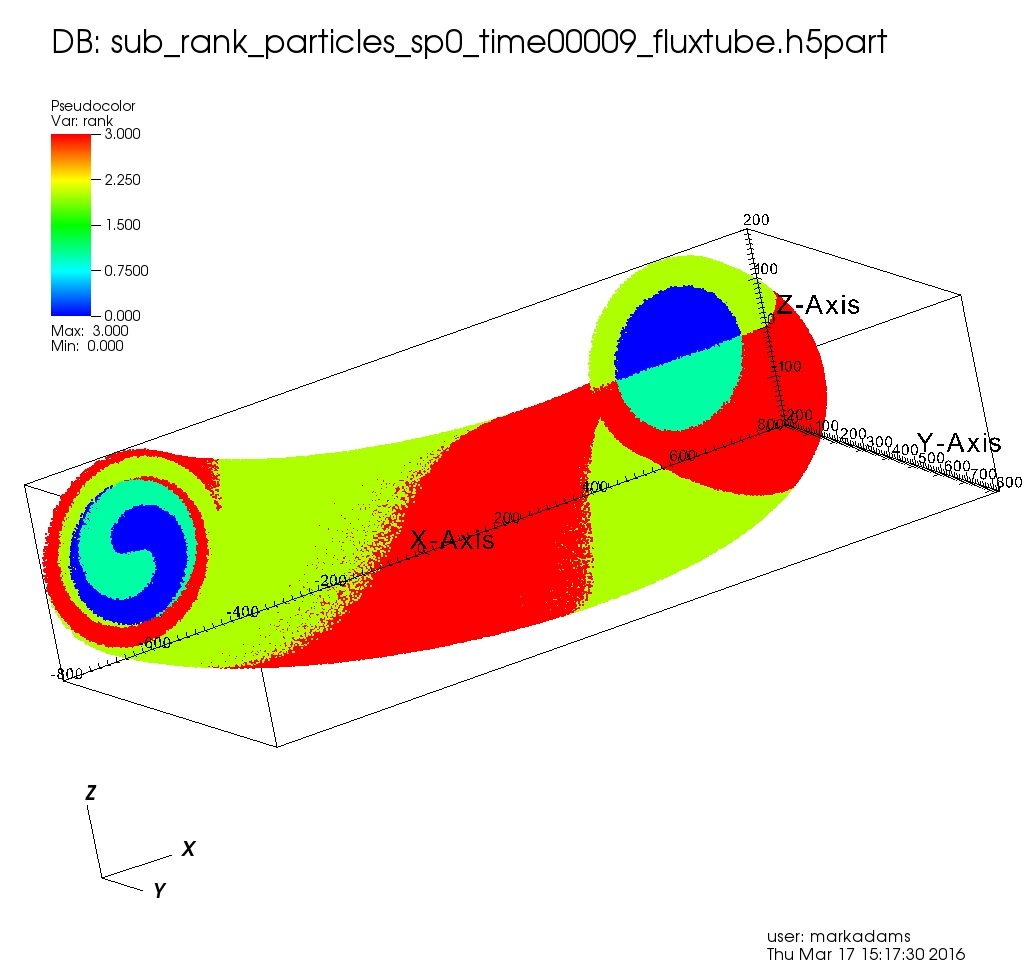
\includegraphics[width=75mm]{half_grid.jpeg} 
    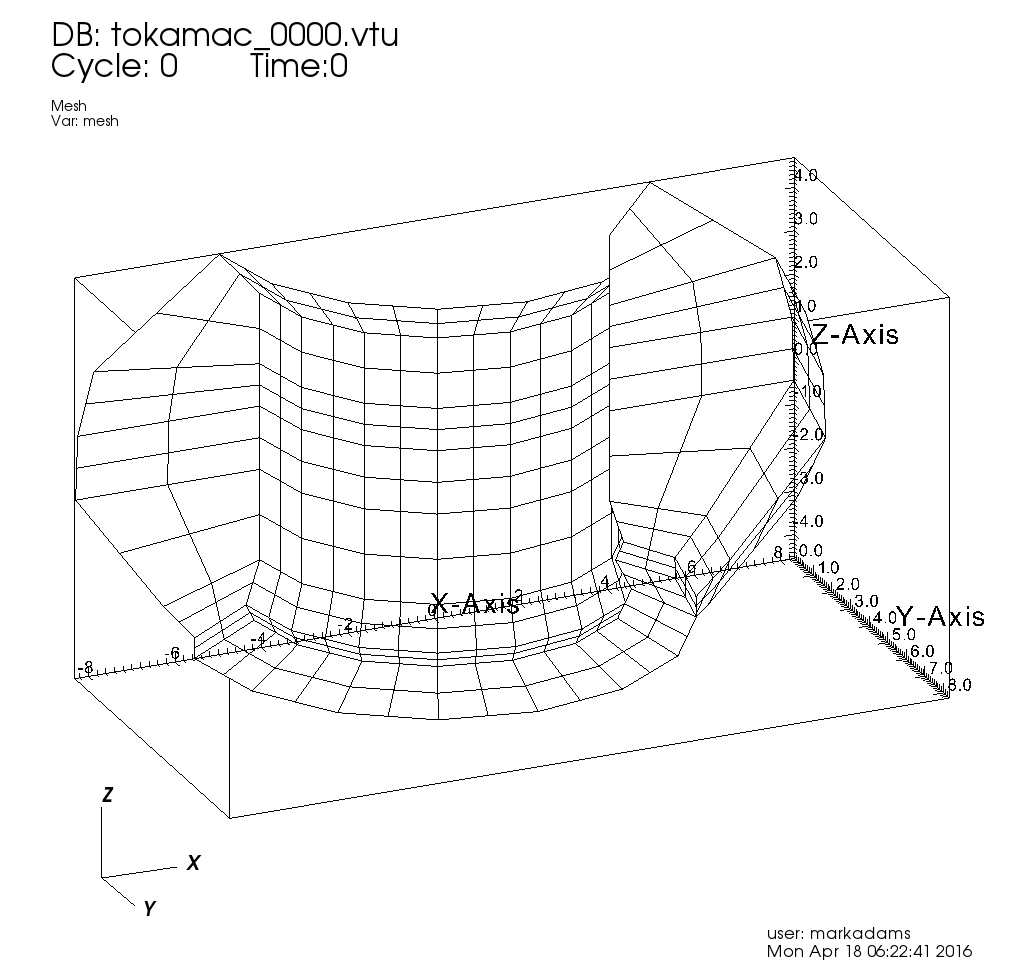
\includegraphics[width=75mm]{half_grid_mesh.jpeg} 
   \caption{Example 2x2x2 flux tube particle partition of torus (left); coarse grid solver mesh (right)}
   \label{fig:cross}
\end{figure}

The fuzzy edges of Figure \ref{fig:cross} (left) are due to the finite number of particles, each particle is drawn with the color of the partition to which it belongs.

\section{Future plans}

The realization of an engineering relevant full plasma simulation of ITER is a significant multi-year undertaking.
The development plans for this project are to be incrementally relevant and engaged with the physics community.
To this end early deliverables are important, to encourage physicists to participate and to stay grounded in the real engineering demands of this enterprise.
To this end we see two early areas that our project can contribute:
\begin{itemize}
\item Explore data decompositions and collect performance data to help further refine effective distributed data models for fusion PIC applications
\item Cross code verification of existing fusion PIC codes, without full physics, but with full ITER wall geometries
\end{itemize}
 
\bibliographystyle{siamplain}
\bibliography{./bib}


 
\end{document}  